\subsection{Completed Single-Host Pilot}
\label{sec:pilot}
On November 17, 2026, we completed 160 independently executed runs on Docker
Desktop 29.2.1, WSL2 kernel 6.6.87.2, twelve logical CPUs and approximately
7.43~GiB of Docker-visible memory. The seeded, randomized schedule used ten
runs per cell: two configurations and four interference scenarios for payments
(80 runs), and two configurations and two scenarios for each Spark workload
(80 runs). Collection, fitting and reporting finished in 4~h 29~min.
Smoke runs used to check execution were excluded.

The shared configuration placed the victim on logical CPUs 4--5 and an
eight-process competing workload on CPUs 4--11. The hardened adaptation
placed the competitor on CPUs 6--11, applied a two-CPU quota per tenant,
dropped capabilities and enabled no-new-privileges. Observer and load-generation
work used CPUs 0--3. This performance-control adaptation is distinct from the
complete security configuration used in E1--E5; it does not repeat their boundary
or integrity tests. Both profiles used the same application and competing work.
Resource allocation and quota effects remain bundled in this pilot.

Payments received 50 requests/s using an open-arrival HTTP driver. Requests
retain scheduled and completed timestamps, including scheduling delay; the first
ten seconds were excluded from request p99. Spark 4.0.1 ran in \code{local[2]}
mode on 20,000 seeded generated rows with eight features. RandomForest used ten
trees and depth five; linear SVM used ten iterations. Dataset initialization was
excluded and successive model-fitting jobs were timed. Spark results summarize
completed-job durations, not request percentiles. Each run retained twelve
five-second telemetry samples over 60~s, followed by a 30~s cooldown.
Payments scenarios were clean, sustained contention, 15~s alternating bursts,
and a competitor on disjoint logical CPUs. The latter is named ``benign'' in
the artifact, but its degradation label comes from measured performance rather
than that scenario name. Spark used clean and sustained-contention scenarios.

\subsection{Common Telemetry and Model Adaptation}
The collector retained sixteen engine/process aggregate features for each of
the victim and competing containers: CPU utilization, memory, process count,
network and I/O rates, throttling, CPU pressure, process CPU and resident memory,
threads, process I/O, and context switches. It required a trusted host-PID
observer, \code{SYS\_PTRACE}, the Docker API, and read-only cgroup access.
Application latency and job time were excluded from detector inputs.
Missing process access failed collection; disappearing processes were skipped.

The neural baseline adapts the architecture documented in the 2024 study
\cite{qos2024}: dense encoder widths 512/256/128, a 20-dimensional sigmoid
bottleneck and mirrored decoder, followed by LSTM layers of 1024/512 units,
dense layers of 512/256 units and two-class softmax. Our input has 32 aggregate
features from two containers, rather than the original 411-feature distributed
service representation. We use train-only min/max scaling clipped to $[0,1]$
for the sigmoid decoder, a six-sample temporal window, and current runtime
libraries. The topology, feature pipeline, workloads, scaling and window policy
are therefore explicit adaptations, not an exact reproduction of the original
method or its published accuracy.

The IsoLab resource-logistic extension uses standard, class-balanced logistic
regression with fixed $C=1$ on the mean of the same six samples, with train-only
standardization. This is an inexpensive engineering alternative, not a new
learning algorithm. Comparators are a validation-selected competing-CPU
threshold and the unchanged DET-08 implementation. DET-08 is positive when its
sustained-sharing event occurs during the run. Learned scores summarize the
last 30~s; the comparison is consequently offline run classification, not
equivalent online detection-delay measurement.

\subsection{Partitions, Labels and Evaluation}
Executions were split 40/30/30 within each cell, with all samples from one run
kept in one partition. Payments has 32 training, 24 validation and 24 test runs;
RF and SVM each have 16/12/12. The run-level positive label is victim time
exceeding 1.2 times the largest clean training-run value for its workload/profile,
or any failed request. Thus injected contention alone is not ground truth.
All runs completed and no request errors were recorded.

The autoencoder minimizes root-mean-square reconstruction loss; the classifier
minimizes cross-entropy. Both use Adam at $10^{-4}$, batch size 512 and at most
1000 epochs. Autoencoder validation patience is ten epochs; classification
patience is twenty, restoring the best validation weights. The autoencoders
reached 1000 epochs; payments/RF/SVM classifiers stopped after 49/117/239 epochs.
Thresholds maximize validation F1, with ties favoring lower FPR and then a
higher threshold. No test-set retuning was performed. Model fitting is measured
once per workload; timing is not a repeated performance benchmark.

\begin{table*}[t]
\caption{Held-out single-host pilot: run-level detection and fitting cost}
\label{tab:pilot}
\centering\small
\begin{tabular}{llrrrrrr}
\toprule
Workload & Method & Test runs & Precision & Recall & F1 & FPR & Fit time (s) \\
\midrule
Payments & Adapted AE/LSTM & 24 & 1.000 & 0.889 & 0.941 & 0.000 & 43.16 \\
Payments & Resource logistic & 24 & 1.000 & 1.000 & 1.000 & 0.000 & 0.01 \\
Payments & CPU threshold & 24 & 1.000 & 0.778 & 0.875 & 0.000 & 0.00 \\
Payments & DET-08 & 24 & 1.000 & 0.333 & 0.500 & 0.000 & 0.00 \\
RF & Adapted AE/LSTM & 12 & 1.000 & 1.000 & 1.000 & 0.000 & 56.55 \\
RF & Resource logistic & 12 & 1.000 & 1.000 & 1.000 & 0.000 & 0.01 \\
RF & CPU threshold & 12 & 1.000 & 1.000 & 1.000 & 0.000 & 0.00 \\
RF & DET-08 & 12 & 1.000 & 1.000 & 1.000 & 0.000 & 0.00 \\
SVM & Adapted AE/LSTM & 12 & 1.000 & 0.750 & 0.857 & 0.000 & 85.78 \\
SVM & Resource logistic & 12 & 1.000 & 0.250 & 0.400 & 0.000 & 0.00 \\
SVM & CPU threshold & 12 & 1.000 & 0.500 & 0.667 & 0.000 & 0.00 \\
SVM & DET-08 & 12 & 1.000 & 0.750 & 0.857 & 0.000 & 0.00 \\
\bottomrule
\end{tabular}
\end{table*}

\begin{figure*}[t]
\centering
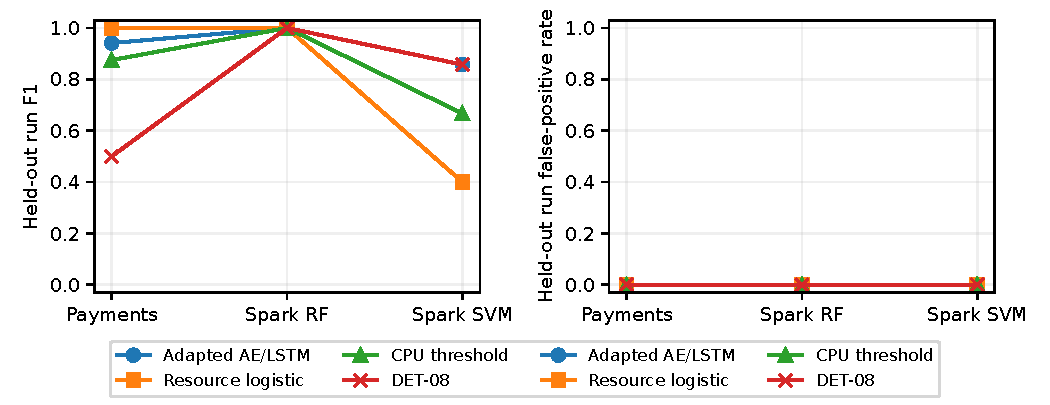
\includegraphics[width=.93\textwidth]{ieee-pilot-detection.pdf}
\caption{Measured held-out run classification using common local telemetry.
Payments has 24 test runs; RF and SVM each have twelve. Zero observed false
positives applies only to the small negative test sets, not to an operational
false-alarm guarantee. Lines connect workload categories for readability.}
\label{fig:pilotdetection}
\end{figure*}

\subsection{Accuracy, Cost and Workload Dependence}
Table~\ref{tab:pilot} and Fig.~\ref{fig:pilotdetection} show the complete matched
comparison. On payments, the resource-logistic model correctly classified all
24 test runs (nine positives, fifteen negatives), yielding F1 1.000; the neural
adaptation missed one bursty run, yielding 0.941. Both have AUC 1.000, illustrating
that validation-selected operating thresholds matter even with identical test
ranking. On RF, all four methods classify three positives and nine negatives
correctly. On SVM, the logistic model detects one of four positives, compared
with three for the neural model and DET-08: F1 is 0.400 versus 0.857.
The lightweight method therefore improves the payments point estimate and ties
RF, but is not consistently more accurate.

No method produced a false positive in these test sets. Negative counts are
only 15/9/8 for payments/RF/SVM. A post-hoc paired run bootstrap (5000 resamples,
excluding undefined F1 draws) gives 95\% intervals for logistic minus neural F1
of $[0,0.231]$, $[0,0]$, and $[-1,0]$, respectively. These conditional intervals
are exploratory, unadjusted for multiple comparisons and limited by the small
sample. The RF interval reflects identical observed predictions, not established
equivalence on future data. The intervals do not establish a general accuracy
advantage.

Logistic fitting took 0.01295/0.00629/0.00330~s for payments/RF/SVM; the neural
pipeline took 43.16/56.55/85.78~s. Batch-amortized inference took approximately
0.00394/0.00533/0.00315~ms per run for logistic regression, compared with
1.623/2.652/2.480~ms for the neural classifier. These timings exclude telemetry
collection and do not measure end-to-end online latency. A production cost claim
also needs repeated timing and a monitoring-disabled comparison.

DET-08's payments F1 of 0.500 follows from its narrower semantics: it missed the
three bursty and three disjoint-CPU competitor positives. A 30~s sustained-sharing
rule is not designed to capture every short burst or every residual source of
degradation. The logistic extension detects those cases in this sample, while
its SVM errors show that replacing DET-08 universally would be unjustified.
These observations answer RQ5 as a workload-dependent accuracy/cost tradeoff.

\subsection{Interference Reduction and Resource Cost}
\begin{table*}[t]
\caption{Sustained-contention pilot: performance benefit and competing-workload cost}
\label{tab:pilotcontrols}
\centering\small
\begin{tabular}{lrrrrrr}
\toprule
Workload & Shared (ms) & Hardened (ms) & Reduction (\%) & Shared bg. & Hardened bg. & Bg. loss (\%) \\
\midrule
PAYMENTS & 10.997 & 4.287 & 61.011 & 98.953 & 34.124 & 65.515 \\
RF & 1103.983 & 716.498 & 35.099 & 89.499 & 31.131 & 65.216 \\
SVM & 901.566 & 539.942 & 40.111 & 88.731 & 31.506 & 64.493 \\
\bottomrule
\end{tabular}
\smallskip
\parbox{.95\textwidth}{\footnotesize Ten independent runs per cell; entries are medians of run summaries. Payments uses request p99; RF and SVM use median completed-job duration. Background (bg.) throughput is completed 100,000-hash batches per second, not tenant requests.}
\end{table*}

\begin{figure*}[t]
\centering
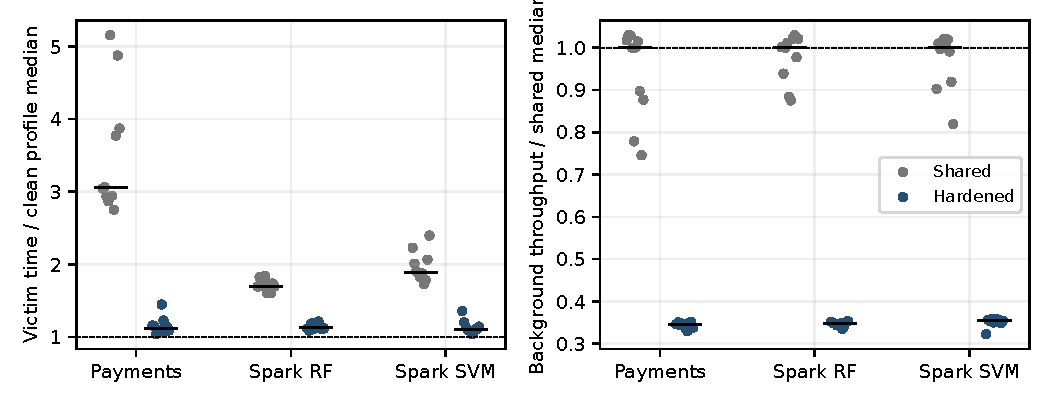
\includegraphics[width=.93\textwidth]{ieee-pilot-controls.pdf}
\caption{Original pilot measurements under sustained contention. Each point is
one run and each black segment is a median. Left: victim time normalized by its
profile's clean median. Right: competing throughput normalized by the shared
configuration's median. Lower victim time accompanies lower competing throughput;
the controls are not a cost-free efficiency improvement.}
\label{fig:pilotcontrols}
\end{figure*}
Under sustained contention, median payments request p99 fell from 10.997 to
4.287~ms (61.0\%); RF job time fell from 1103.983 to 716.498~ms (35.1\%);
and SVM job time fell from 901.566 to 539.942~ms (40.1\%). Each cell has ten
independent runs. These are within-testbed configuration effects, not improvements
over the 2024 detector, which is a monitoring method rather than this control arm.
Table~\ref{tab:pilotcontrols} reports the competing-workload throughput loss
alongside those gains. Restricting the competitor to two CPUs reduces its completed
hash-batch throughput by approximately 64--66\%. A provider must weigh protection
of the victim against the reduced service available to competing tenants.

\subsection{Implications for Further Improvement}
The strongest supported result is an inspectable combination of resource
protection, inexpensive workload-specific classification and security evidence.
Improvement should next target robust operating points and workload diversity:
use additional validation executions to assess threshold sensitivity, retain
CPU-sharing rules as complementary evidence, and test a burst-aware policy on
new held-out data. Model selection or hybrid routing based on the present SVM
test errors would require a new independent evaluation. Longer runs, unseen
datasets, workload churn, individual-control ablations and multi-host experiments
are needed before a general improvement over the source method can be claimed.
